\documentclass[]{article}
\usepackage{amssymb,amsmath}
\usepackage{ifxetex,ifluatex}
\ifxetex
  \usepackage{fontspec,xltxtra,xunicode}
  \defaultfontfeatures{Mapping=tex-text,Scale=MatchLowercase}
\else
  \ifluatex
    \usepackage{fontspec}
    \defaultfontfeatures{Mapping=tex-text,Scale=MatchLowercase}
  \else
    \usepackage[utf8]{inputenc}
  \fi
\fi
\usepackage{ctable}
\usepackage{float} % provides the H option for float placement
\usepackage{graphicx}
% We will generate all images so they have a width \maxwidth. This means
% that they will get their normal width if they fit onto the page, but
% are scaled down if they would overflow the margins.
\makeatletter
\def\maxwidth{\ifdim\Gin@nat@width>\linewidth\linewidth
\else\Gin@nat@width\fi}
\makeatother
\let\Oldincludegraphics\includegraphics
\renewcommand{\includegraphics}[1]{\Oldincludegraphics[width=\maxwidth]{#1}}
\ifxetex
  \usepackage[setpagesize=false, % page size defined by xetex
              unicode=false, % unicode breaks when used with xetex
              xetex,
              colorlinks=true,
              linkcolor=blue]{hyperref}
\else
  \usepackage[unicode=true,
              colorlinks=true,
              linkcolor=blue]{hyperref}
\fi
\hypersetup{breaklinks=true, pdfborder={0 0 0}}
\newcommand{\textsubscr}[1]{\ensuremath{_{\scriptsize\textrm{#1}}}}
\setlength{\parindent}{0pt}
\setlength{\parskip}{6pt plus 2pt minus 1pt}
\setlength{\emergencystretch}{3em}  % prevent overfull lines
\setcounter{secnumdepth}{0}

\title{Normality Tests}
\author{Rapport package team @ https://github.com/aL3xa/rapport}
\date{2011-04-26 20:25 CET}

\begin{document}
\maketitle

\subsection{Description}

Overview of several normality tests and diagnostic plots that can screen
departures from normality.

\subsection{Introduction}

In statistics, \emph{normality} refers to an assumption that the
distribution of a random variable follows \emph{normal}
(\emph{Gaussian}) distribution. Because of its bell-like shape, it's
also known as the \emph{``bell curve''}. The formula for \emph{normal
distribution} is:

\[f(x) = \frac{1}{\sqrt{2\pi{}\sigma{}^2}} e^{-\frac{(x-\mu{})^2}{2\sigma{}^2}}\]

\emph{Normal distribution} belongs to a \emph{location-scale family} of
distributions, as it's defined two parameters:

\begin{itemize}
\item
  \emph{μ} - \emph{mean} or \emph{expectation} (location parameter)
\item
  \emph{σ\textsuperscript{2}} - \emph{variance} (scale parameter)
\end{itemize}
\href{806ea97c59e1a12d4acae4968957aaa9-hires.png}{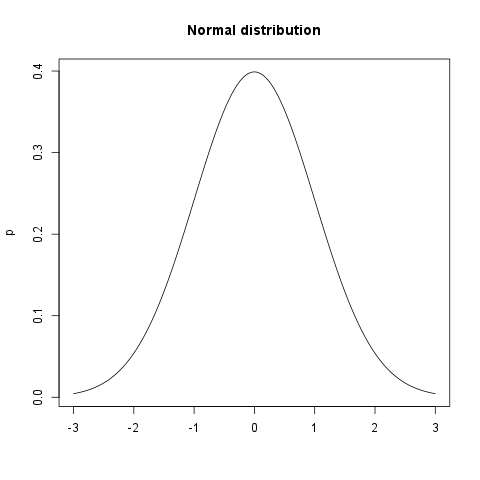
\includegraphics{806ea97c59e1a12d4acae4968957aaa9.png}}

\subsection{Normality Tests}

\subsubsection{Overview}

Various hypothesis tests can be applied in order to test if the
distribution of given random variable violates normality assumption.
These procedures test the H\textsubscr{0} that provided variable's
distribution is \emph{normal}. At this point only few such tests will be
covered: the ones that are available in \texttt{stats} package (which
comes bundled with default R installation) and \texttt{nortest} package
that is
\href{http://cran.r-project.org/web/packages/nortest/index.html}{available}
on CRAN.

\begin{itemize}
\item
  \textbf{Shapiro-Wilk test} is a powerful normality test appropriate
  for small samples. In R, it's implemented in \texttt{shapiro.test}
  function available in \texttt{stats} package.
\item
  \textbf{Lilliefors test} is a modification of \emph{Kolmogorov-Smirnov
  test} appropriate for testing normality when parameters or normal
  distribution (\emph{μ}, \emph{σ\textsuperscript{2}}) are not known.
  \texttt{lillie.test} function is located in \texttt{nortest} package.
\item
  \textbf{Anderson-Darling test} is one of the most powerful normality
  tests as it will detect the most of departures from normality. You can
  find \texttt{ad.test} function in \texttt{nortest} package.
\item
  \textbf{Pearson Χ\textsuperscript{2} test} is another normality test
  which takes more ``traditional'' approach in normality testing.
  \texttt{pearson.test} is located in \texttt{nortest} package.
\end{itemize}
\subsubsection{Results}

Here you can see the results of applied normality tests (\emph{p-values}
less than 0.05 indicate significant discrepancies):

\ctable[pos = H, center, botcap]{lll}
{% notes
}
{% rows
\FL
 & \textbf{Statistic} & \textbf{p-value}
\ML
Shapiro-Wilk normality test & 0.9001 & 0
\\\noalign{\medskip}
Lilliefors (Kolmogorov-Smirnov) normality test & 0.168 & 0
\\\noalign{\medskip}
Anderson-Darling normality test & 18.753 & 0
\\\noalign{\medskip}
Pearson chi-square normality test & 1791.25 & 0
\LL
}

So, let's draw some conclusions based on applied normality test:

\begin{itemize}
\item
  according to \emph{Shapiro-Wilk test}, the distribution of
  \emph{Internet usage in leisure time (hours per day)} is not normal.
\item
  based on \emph{Lilliefors test}, distribution of \emph{Internet usage
  in leisure time (hours per day)} is not normal
\item
  \emph{Anderson-Darling test} confirms violation of normality
  assumption
\item
  \emph{Pearson's Χ\textsuperscript{2} test} classifies the underlying
  distribution as normal
\end{itemize}
\subsection{Diagnostic Plots}

There are various plots that can help you decide about the normality of
the distribution. Only a few most commonly used plots will be shown:
\emph{histogram}, \emph{Q-Q plot} and \emph{kernel density plot}.

\subsubsection{Histogram}

\emph{Histogram} was first introduced by \emph{Karl Pearson} and it's
probably the most popular plot for depicting the probability
distribution of a random variable. However, the decision depends on
number of bins, so it can sometimes be misleading. If the variable
distribution is normal, bins should resemble the ``bell-like'' shape.

\href{a949c4cf7eda15cd079e9d63b81acdd4-hires.png}{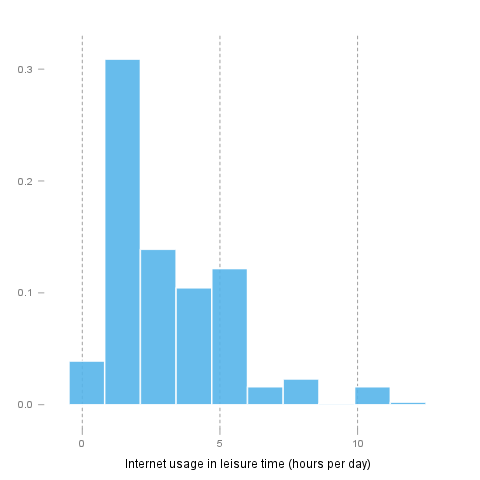
\includegraphics{a949c4cf7eda15cd079e9d63b81acdd4.png}}

\subsubsection{Q-Q Plot}

``Q'' in \emph{Q-Q plot} stands for \emph{quantile}, as this plot
compares empirical and theoretical distribution (in this case,
\emph{normal} distribution) by plotting their quantiles against each
other. For normal distribution, plotted dots should approximate a
``straight'', \texttt{x = y} line.

\href{eecb9a780afd4dd0de9737991e467a6e-hires.png}{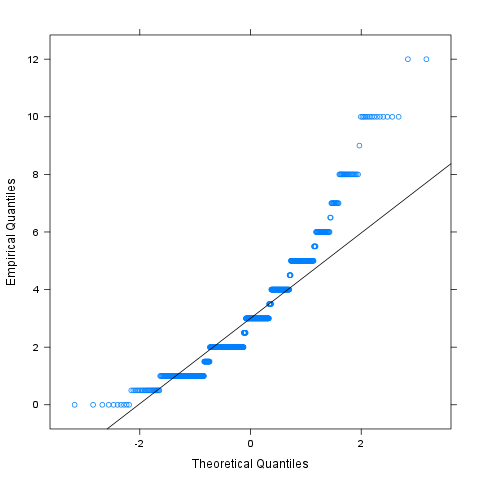
\includegraphics{eecb9a780afd4dd0de9737991e467a6e.png}}

\subsubsection{Kernel Density Plot}

\emph{Kernel density plot} is a plot of smoothed \emph{empirical
distribution function}. As such, it provides good insight about the
shape of the distribution. For normal distributions, it should resemble
the well known ``bell shape''.

\href{fe4ddb2fb2ffd78d3c5448a9cc27a8de-hires.png}{\includegraphics{fe4ddb2fb2ffd78d3c5448a9cc27a8de.png}}

\subsection{Description}

Overview of several normality tests and diagnostic plots that can screen
departures from normality.

\subsection{Introduction}

In statistics, \emph{normality} refers to an assumption that the
distribution of a random variable follows \emph{normal}
(\emph{Gaussian}) distribution. Because of its bell-like shape, it's
also known as the \emph{``bell curve''}. The formula for \emph{normal
distribution} is:

\[f(x) = \frac{1}{\sqrt{2\pi{}\sigma{}^2}} e^{-\frac{(x-\mu{})^2}{2\sigma{}^2}}\]

\emph{Normal distribution} belongs to a \emph{location-scale family} of
distributions, as it's defined two parameters:

\begin{itemize}
\item
  \emph{μ} - \emph{mean} or \emph{expectation} (location parameter)
\item
  \emph{σ\textsuperscript{2}} - \emph{variance} (scale parameter)
\end{itemize}
\subsection{Normality Tests}

\subsubsection{Overview}

Various hypothesis tests can be applied in order to test if the
distribution of given random variable violates normality assumption.
These procedures test the H\textsubscr{0} that provided variable's
distribution is \emph{normal}. At this point only few such tests will be
covered: the ones that are available in \texttt{stats} package (which
comes bundled with default R installation) and \texttt{nortest} package
that is
\href{http://cran.r-project.org/web/packages/nortest/index.html}{available}
on CRAN.

\begin{itemize}
\item
  \textbf{Shapiro-Wilk test} is a powerful normality test appropriate
  for small samples. In R, it's implemented in \texttt{shapiro.test}
  function available in \texttt{stats} package.
\item
  \textbf{Lilliefors test} is a modification of \emph{Kolmogorov-Smirnov
  test} appropriate for testing normality when parameters or normal
  distribution (\emph{μ}, \emph{σ\textsuperscript{2}}) are not known.
  \texttt{lillie.test} function is located in \texttt{nortest} package.
\item
  \textbf{Anderson-Darling test} is one of the most powerful normality
  tests as it will detect the most of departures from normality. You can
  find \texttt{ad.test} function in \texttt{nortest} package.
\item
  \textbf{Pearson Χ\textsuperscript{2} test} is another normality test
  which takes more ``traditional'' approach in normality testing.
  \texttt{pearson.test} is located in \texttt{nortest} package.
\end{itemize}
\subsubsection{Results}

Here you can see the results of applied normality tests (\emph{p-values}
less than 0.05 indicate significant discrepancies):

\ctable[pos = H, center, botcap]{lll}
{% notes
}
{% rows
\FL
 & \textbf{Statistic} & \textbf{p-value}
\ML
Shapiro-Wilk normality test & 0.9001 & 0
\\\noalign{\medskip}
Lilliefors (Kolmogorov-Smirnov) normality test & 0.168 & 0
\\\noalign{\medskip}
Anderson-Darling normality test & 18.753 & 0
\\\noalign{\medskip}
Pearson chi-square normality test & 1791.25 & 0
\LL
}

So, let's draw some conclusions based on applied normality test:

\begin{itemize}
\item
  according to \emph{Shapiro-Wilk test}, the distribution of
  \emph{Internet usage in leisure time (hours per day)} is not normal.
\item
  based on \emph{Lilliefors test}, distribution of \emph{Internet usage
  in leisure time (hours per day)} is not normal
\item
  \emph{Anderson-Darling test} confirms violation of normality
  assumption
\item
  \emph{Pearson's Χ\textsuperscript{2} test} classifies the underlying
  distribution as normal
\end{itemize}
\subsection{Diagnostic Plots}

There are various plots that can help you decide about the normality of
the distribution. Only a few most commonly used plots will be shown:
\emph{histogram}, \emph{Q-Q plot} and \emph{kernel density plot}.

\subsubsection{Histogram}

\emph{Histogram} was first introduced by \emph{Karl Pearson} and it's
probably the most popular plot for depicting the probability
distribution of a random variable. However, the decision depends on
number of bins, so it can sometimes be misleading. If the variable
distribution is normal, bins should resemble the ``bell-like'' shape.

\href{a949c4cf7eda15cd079e9d63b81acdd4-hires.png}{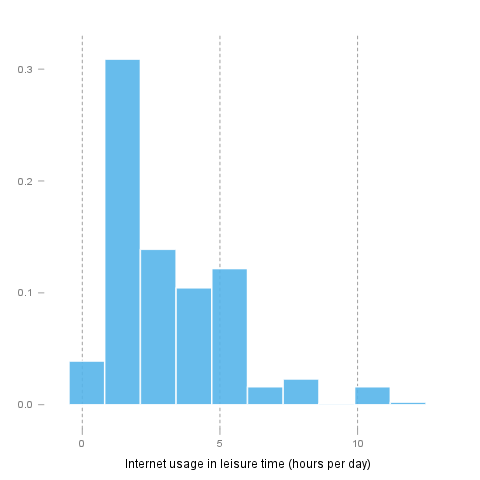
\includegraphics{a949c4cf7eda15cd079e9d63b81acdd4.png}}

\subsubsection{Q-Q Plot}

``Q'' in \emph{Q-Q plot} stands for \emph{quantile}, as this plot
compares empirical and theoretical distribution (in this case,
\emph{normal} distribution) by plotting their quantiles against each
other. For normal distribution, plotted dots should approximate a
``straight'', \texttt{x = y} line.

\href{eecb9a780afd4dd0de9737991e467a6e-hires.png}{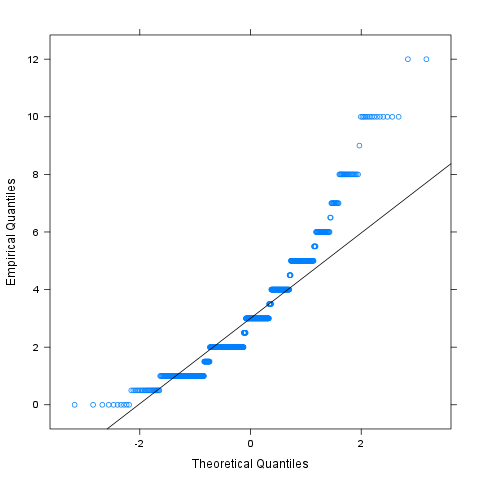
\includegraphics{eecb9a780afd4dd0de9737991e467a6e.png}}

\subsubsection{Kernel Density Plot}

\emph{Kernel density plot} is a plot of smoothed \emph{empirical
distribution function}. As such, it provides good insight about the
shape of the distribution. For normal distributions, it should resemble
the well known ``bell shape''.

\href{daf251be0fc0a31c9b51a510640ce60f-hires.png}{\includegraphics{daf251be0fc0a31c9b51a510640ce60f.png}}

\subsection{Description}

Overview of several normality tests and diagnostic plots that can screen
departures from normality.

\subsection{Introduction}

In statistics, \emph{normality} refers to an assumption that the
distribution of a random variable follows \emph{normal}
(\emph{Gaussian}) distribution. Because of its bell-like shape, it's
also known as the \emph{``bell curve''}. The formula for \emph{normal
distribution} is:

\[f(x) = \frac{1}{\sqrt{2\pi{}\sigma{}^2}} e^{-\frac{(x-\mu{})^2}{2\sigma{}^2}}\]

\emph{Normal distribution} belongs to a \emph{location-scale family} of
distributions, as it's defined two parameters:

\begin{itemize}
\item
  \emph{μ} - \emph{mean} or \emph{expectation} (location parameter)
\item
  \emph{σ\textsuperscript{2}} - \emph{variance} (scale parameter)
\end{itemize}
\href{806ea97c59e1a12d4acae4968957aaa9-hires.png}{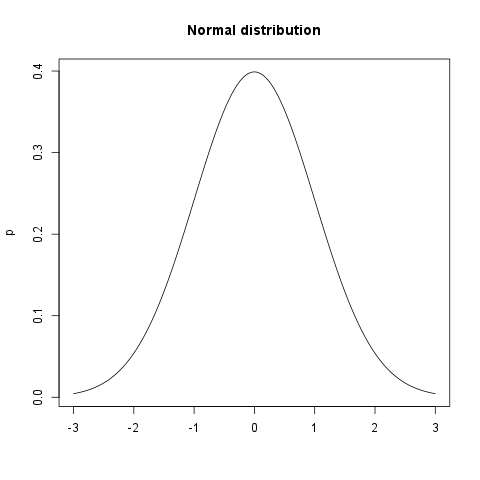
\includegraphics{806ea97c59e1a12d4acae4968957aaa9.png}}

\subsection{Normality Tests}

\subsubsection{Overview}

Various hypothesis tests can be applied in order to test if the
distribution of given random variable violates normality assumption.
These procedures test the H\textsubscr{0} that provided variable's
distribution is \emph{normal}. At this point only few such tests will be
covered: the ones that are available in \texttt{stats} package (which
comes bundled with default R installation) and \texttt{nortest} package
that is
\href{http://cran.r-project.org/web/packages/nortest/index.html}{available}
on CRAN.

\begin{itemize}
\item
  \textbf{Shapiro-Wilk test} is a powerful normality test appropriate
  for small samples. In R, it's implemented in \texttt{shapiro.test}
  function available in \texttt{stats} package.
\item
  \textbf{Lilliefors test} is a modification of \emph{Kolmogorov-Smirnov
  test} appropriate for testing normality when parameters or normal
  distribution (\emph{μ}, \emph{σ\textsuperscript{2}}) are not known.
  \texttt{lillie.test} function is located in \texttt{nortest} package.
\item
  \textbf{Anderson-Darling test} is one of the most powerful normality
  tests as it will detect the most of departures from normality. You can
  find \texttt{ad.test} function in \texttt{nortest} package.
\item
  \textbf{Pearson Χ\textsuperscript{2} test} is another normality test
  which takes more ``traditional'' approach in normality testing.
  \texttt{pearson.test} is located in \texttt{nortest} package.
\end{itemize}
\subsubsection{Results}

Here you can see the results of applied normality tests (\emph{p-values}
less than 0.05 indicate significant discrepancies):

\ctable[pos = H, center, botcap]{lll}
{% notes
}
{% rows
\FL
 & \textbf{Statistic} & \textbf{p-value}
\ML
Shapiro-Wilk normality test & 0.9001 & 0
\\\noalign{\medskip}
Lilliefors (Kolmogorov-Smirnov) normality test & 0.168 & 0
\\\noalign{\medskip}
Anderson-Darling normality test & 18.753 & 0
\\\noalign{\medskip}
Pearson chi-square normality test & 1791.25 & 0
\LL
}

So, let's draw some conclusions based on applied normality test:

\begin{itemize}
\item
  according to \emph{Shapiro-Wilk test}, the distribution of
  \emph{Internet usage in leisure time (hours per day)} is not normal.
\item
  based on \emph{Lilliefors test}, distribution of \emph{Internet usage
  in leisure time (hours per day)} is not normal
\item
  \emph{Anderson-Darling test} confirms violation of normality
  assumption
\item
  \emph{Pearson's Χ\textsuperscript{2} test} classifies the underlying
  distribution as normal
\end{itemize}
\subsection{Diagnostic Plots}

There are various plots that can help you decide about the normality of
the distribution. Only a few most commonly used plots will be shown:
\emph{histogram}, \emph{Q-Q plot} and \emph{kernel density plot}.

\subsubsection{Histogram}

\emph{Histogram} was first introduced by \emph{Karl Pearson} and it's
probably the most popular plot for depicting the probability
distribution of a random variable. However, the decision depends on
number of bins, so it can sometimes be misleading. If the variable
distribution is normal, bins should resemble the ``bell-like'' shape.

\href{a949c4cf7eda15cd079e9d63b81acdd4-hires.png}{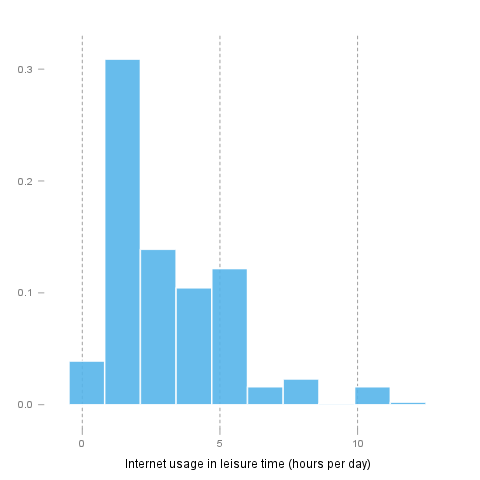
\includegraphics{a949c4cf7eda15cd079e9d63b81acdd4.png}}

\subsubsection{Q-Q Plot}

``Q'' in \emph{Q-Q plot} stands for \emph{quantile}, as this plot
compares empirical and theoretical distribution (in this case,
\emph{normal} distribution) by plotting their quantiles against each
other. For normal distribution, plotted dots should approximate a
``straight'', \texttt{x = y} line.

\href{95d42d4d0934008cfa630e1c4523e09a-hires.png}{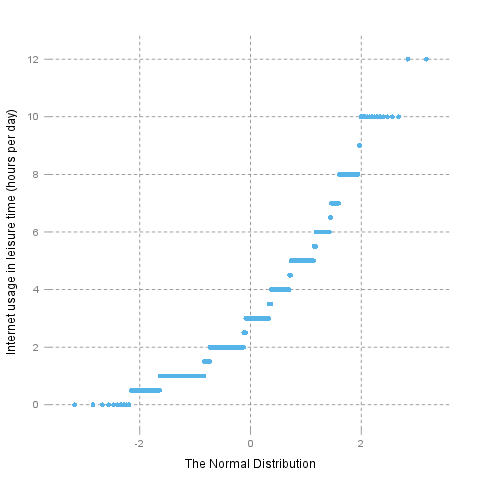
\includegraphics{95d42d4d0934008cfa630e1c4523e09a.png}}

\subsubsection{Kernel Density Plot}

\emph{Kernel density plot} is a plot of smoothed \emph{empirical
distribution function}. As such, it provides good insight about the
shape of the distribution. For normal distributions, it should resemble
the well known ``bell shape''.

\href{db1e16796e7e791e46cc0c0ca2f68bab-hires.png}{\includegraphics{db1e16796e7e791e46cc0c0ca2f68bab.png}}

\begin{center}\rule{3in}{0.4pt}\end{center}

This report was generated with \href{http://www.r-project.org/}{R}
(2.14.0) and \href{http://al3xa.github.com/rapport/}{rapport} (0.2) in
2.928 sec on x86\_64-unknown-linux-gnu platform.

\begin{figure}[htbp]
\centering

\includegraphics{images/logo.png}
\caption{}
\end{figure}

\end{document}
